\documentclass[border=10pt,varwidth=\maxdimen]{standalone}

\usepackage{verbatim}
\usepackage{tikz}
\usetikzlibrary{calc, shapes, backgrounds,graphs,positioning,fit}
\usetikzlibrary{bayesnet}
\usetikzlibrary{arrows}

\usepackage{amsmath, amssymb}
\usepackage{graphicx}

\begin{document}
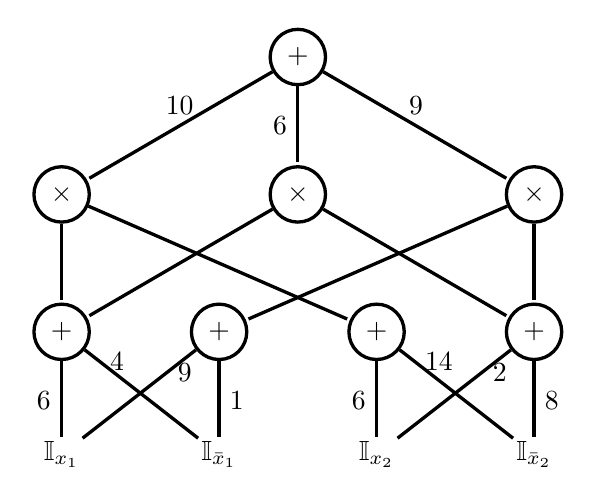
\begin{tikzpicture}[>=stealth',shorten >=1pt,auto,node distance=3cm, very thick]
    \node (root) [latent] {$+$};
    \node (P1) [latent, below=of root, xshift=-3cm] {$\times$};
    \node (P2) [latent, below=of root] {$\times$};
    \node (P3) [latent, below=of root, xshift=3cm] {$\times$};

    \node (S1) [latent, below=of P1] {$+$};
    \node (S2) [latent, below=of P2, xshift=-1cm] {$+$};
    \node (S3) [latent, below=of P2, xshift=1cm] {$+$};
    \node (S4) [latent, below=of P3] {$+$};

    \node (I1) [const, below=of S1] {$\mathbb{I}_{x_1}$};
    \node (I2) [const, below=of S2] {$\mathbb{I}_{\bar{x}_1}$};
    \node (I3) [const, below=of S3] {$\mathbb{I}_{x_2}$};
    \node (I4) [const, below=of S4] {$\mathbb{I}_{\bar{x}_2}$};

    % Create edge connections
    \draw (root) -- (P1) node[left, midway, above] {$10$};
    \draw (root) -- (P2) node[left, midway] {$6$};
    \draw (root) -- (P3) node[right,midway, above] {$9$};

    \draw (P1) -- (S1);
    \draw (P1) -- (S3);
    \draw (P2) -- (S1);
    \draw (P2) -- (S4);
    \draw (P3) -- (S2);
    \draw (P3) -- (S4);

    \draw (S1) -- (I1) node[midway, left] {$6$};
    \draw (S1) -- (I2) node[very near start, right] {$4$};
    \draw (S2) -- (I1) node[near start, right] {$9$};
    \draw (S2) -- (I2) node[midway, right] {$1$};

    \draw (S3) -- (I3) node[midway, left] {$6$};
    \draw (S3) -- (I4) node[very near start, right] {$14$};
    \draw (S4) -- (I3) node[near start, right] {$2$};
    \draw (S4) -- (I4) node[midway, right] {$8$};
\end{tikzpicture}
\end{document}
